% arara: pdflatex
% arara: pdflatex
% arara: pdflatex

% options:
% thesis=B bachelor's thesis
% thesis=M master's thesis
% czech thesis in Czech language
% slovak thesis in Slovak language
% english thesis in English language
% hidelinks remove colour boxes around hyperlinks

\documentclass[thesis=B,czech]{FITthesis}[2012/06/26]

\usepackage[utf8]{inputenc} % LaTeX source encoded as UTF-8

\usepackage{graphicx} %graphics files inclusion
% \usepackage{amsmath} %advanced maths
% \usepackage{amssymb} %additional math symbols

\usepackage{dirtree} %directory tree visualisation

\usepackage[shortlabels]{enumitem}

% % list of acronyms
% \usepackage[acronym,nonumberlist,toc,numberedsection=autolabel]{glossaries}
% \iflanguage{czech}{\renewcommand*{\acronymname}{Seznam pou{\v z}it{\' y}ch zkratek}}{}
% \makeglossaries

\newcommand{\tg}{\mathop{\mathrm{tg}}} %cesky tangens
\newcommand{\cotg}{\mathop{\mathrm{cotg}}} %cesky cotangens

% % % % % % % % % % % % % % % % % % % % % % % % % % % % % % 
% ODTUD DAL VSE ZMENTE
% % % % % % % % % % % % % % % % % % % % % % % % % % % % % % 

\department{Katedra softwarového inženýrství}
\title{Webová aplikace pro online web scraping}
\authorGN{Jakub} %(křestní) jméno (jména) autora
\authorFN{Drahoš} %příjmení autora
\authorWithDegrees{Jakub Drahoš} %jméno autora včetně současných akademických titulů
\author{Jakub Drahoš} %jméno autora bez akademických titulů
\supervisor{Martin Podloucký}
\acknowledgements{Doplňte, máte-li komu a za co děkovat. V~opačném případě úplně odstraňte tento příkaz.}
\abstractCS{V~několika větách shrňte obsah a přínos této práce v~češtině. Po přečtení abstraktu by se čtenář měl mít čtenář dost informací pro rozhodnutí, zda chce Vaši práci číst.}
\abstractEN{Sem doplňte ekvivalent abstraktu Vaší práce v~angličtině.}
\placeForDeclarationOfAuthenticity{V~Praze}
\declarationOfAuthenticityOption{4} %volba Prohlášení (číslo 1-6)
\keywordsCS{web scraping, extrakce dat, aplikace, JavaScript, rozšíření do Chromu}
\keywordsEN{web scraping, data extraction, application, JavaScript, Chrome extension}
% \website{http://site.example/thesis} %volitelná URL práce, objeví se v tiráži - úplně odstraňte, nemáte-li URL práce

\begin{document}

% \newacronym{CVUT}{{\v C}VUT}{{\v C}esk{\' e} vysok{\' e} u{\v c}en{\' i} technick{\' e} v Praze}
% \newacronym{FIT}{FIT}{Fakulta informa{\v c}n{\' i}ch technologi{\' i}}

\begin{introduction}
	\section*{Cíle práce}
	Hlavním cílem této práce je návrh a tvorba webové aplikace, která bude umožňovat uživatelům extrahovat požadovaná data z~libovolné stránky v~reálném čase bez jakékoli nutné znalosti programování. Při specifikaci požadavků tohoto softwaru se přihlídne k analýze stávajících řešení, jež je vedlejším cílem této práce. Druhým vedlejším cílem je poskytnout čtenáři úvod do právní problematiky web scrapingu a shrnout na jednom místě fakta, která máme k dispozici.
	
	Neméně důležitou součást práce tvoří dodržení klasického vývojového cyklu softwarového projektu -- analýza, design, implementace a testování.
	
	Klíčovým aspektem aplikace je též \emph{přehlednost a jednoduchost uživatelského rozhraní} -- důraz bude kladen na intuitivní a rychlé ovládání.
	
	Naopak v rozsahu této práce není tvorba web crawlera ani žádného jiného podobného mechanismu, jenž by systematicky a především \emph{automatizovaně} procházel danou oblast webu.
	
	\section*{Motivace}
	Téma web scrapingu je v dnešní době velice aktuální a čím více dat produkujeme, tím více bude stoupat potřeba tyto informace určitým způsobem získávat a zpracovávat. Téměř kdokoli, kdo pracuje s daty dostupnými z internetu, bude nucen využít nějaký nástroj k vytěžování, aby byl vůbec schopný udržet krok s konkurencí.
	
	Tedy důvod k vytvoření softwaru umožňující extrahovat data z webových stránek je jasný. Ač podobných nástrojů existuje několik, jejich obsluha je poměrně složitá a je nutné strávit určitý čas, než se člověk seznámí s jejich fungováním a může je naplno využít. Právě tento aspekt se snaží aplikace vyvíjená v rámci této bakalářské práce eliminovat -- motivací je tak poskytnout uživatelům možnost jednoduše a rychle vytěžit požadovaná data bez zbytečného zdržování a dlouhého času stráveného seznamováním se s nástrojem.
	
	Jak již bylo řečeno, přínos aplikace spočívá především v její jednoduchosti. Z toho mohou těžit uživatelé, kteří se nezabývají programováním nebo tvorbou webových stránek. Využije ji tak kdokoli, kdo potřebuje jednorázově získat data z libovolné internetové stránky, která obsahuje velké množství dat pohromadě na jedno místě. Z důvodu prozatím chybějícího crawlingu (automatizovaného procházení) je naopak nevhodná k pravidelnému získávání dat (jako je například dlouhodobé sledování cen produktů) či ke zpracování stránek, kdy se jednotlivá data nacházejí rozptýlená po celé doméně.
	
	\section*{Členění práce}
	Kapitola 1 je věnována analýze tématiky web scrapingu. První sekce shrnuje obecné informace, následuje pohled z právní strany věci a nakonec analýza stávajících řešení problému. Kapitola 2 se zaměřuje na návrh aplikace -- specifikace požadavků, architektura systému, návrh uživatelského rozhraní. Ve 3. kapitole je popsána realizace daného návrhu, výběr použitých technologií a odůvodnění rozhodnutí, která byla učiněna. Poslední kapitola je věnovaná testování celé aplikace.
\end{introduction}


% ================================================================================================


\chapter{Analýza}

% ------------------------------------------------------------------------------------------------

\section{Web scraping}
\uv{\textit{Web scraping (nebo také web harvesting, web data extraction) je softwarová technika zaměřená na extrakci informací z webových stránek}}\cite[překlad autora]{web_scraping_def}. Nejčastěji se v~tomto kontextu jedná o~automatizovaný proces strojového zpracování a získávání dat, nicméně může jít i o~manuální extrakci zadanou uživatelem skrze nějaký software (jako je tomu právě v~našem případě).

Často se také v~souvislosti s~pojmem web scraping používá spojení \emph{web crawler} (nebo také \emph{bot, spider, spiderbot}). Jedná se o~automatizovaný software, který systematicky prochází danou oblast webu a během toho vytěžuje kýžená data.\cite{web_crawler_def}

\subsection{Krátce z~historie}
Historie web scrapingu sahá k~samým počátkům internetu (World Wide Web, 1989). Prvním webovým robotem, který byl vyvinut na MIT k~měření velikosti webu, byl World Wide Web Wanderer (napsaný v~jazyce Perl) z~roku 1993.\cite{web_wanderer}

O~něco později, v~roce 2000, se ve velkém začala používat webová APIs -- lidé mohli získávat čistá data přímo od serveru a scraping se tak stal o~hodně jednodušším. Dalším milníkem v~historii web scrapingu je rok 2004, kdy byla vydána knihovna pro parsování HTML a XML dokumentů Beautiful Soup pro programovací jazyk Python. Ta je do dnes považována za nejsofistikovanější a nejpokročilejší knihovnu pro web scraping. Za zmínku stojí určitě i rok 2006, kdy je datován příchod vizuálního web scrapingu, tedy techniky, kdy uživatel skrze rozhraní aplikace označí klikáním myši, z~kterých oblastí webové stránky chce extrahovat data. Tímto se otevřely dveře web scrapingu pro všechny.\cite{web_scraping_history}

\subsection{Techniky}
Technik, jak z~webové stránky získat data existuje mnoho, podívejme se alespoň na některé z~nich:
\begin{itemize}
	\item vyhledávání na základě textové shody -- např. pomocí UNIX nástroje grep nebo regulárních výrazů
	\item HTML parsování -- základní a stále ještě nejpoužívanější technika extrakce dat; informace jednoduše získáváme z~HTML elementů, popř. pomocí tříd nebo id
	\item počítačové vidění, strojové učení, zapojení umělé inteligence -- snaha napodobit způsob, jakým vidí a zpracovává webovou stránku člověk; podobný přístup zkouší např. projekt Diffbot \cite{computer_vision}
	\item vizuální web scraping -- jak již bylo zmíněno výše, požadovaná data se musí ručně naklikat skrze rozhraní nějaké aplikace (značně to však usnadňuje např. hledání podobných prvků na základě prvních pár kliknutí)
	\item manuální vyhledávání a stahování dat (někdy nazývané také \emph{copy--paste})
\end{itemize}

\subsection{Využití web scrapingu}
Podob pro uplatnění scrapování dat z~webu je nespočet, a to obzvlášť v~dnešní době, kdy se dle \cite{data_size} velikost všech dat na celém internetu pohybuje v~řádech Zettabajtů ($1024^{7}$ B). Mezi ty hlavní patří:
\begin{itemize}
	\item získání kontaktních informací (např. e-mail) pro marketingové účely
	\item indexování webových stránek (jako příklad můžeme uvést známý GoogleBot)
	\item data mining -- proces hledání vzorců ve velkých datových setech \cite{data_mining}
	\item monitorování různých proměnných (např. sledování cen nebo hodnocení produktů)
	\item recyklace již někdy použitých dat za účelem vytváření \uv{nového} obsahu
	\item analýza a zpracování dat k~výzkumným účelům
\end{itemize}

% ------------------------------------------------------------------------------------------------

\section{Právní aspekt}
\label{sec:pravni_aspekt}
Podrobná právní analýza celé problematiky web scrapingu by vydala na samostatnou diplomovou práci, a tak se pokusím pouze shrnout základní body, představit hlavní právní pojmy a poskytnout čtenáři alespoň náhled do této oblasti. 

Při získávání dat z internetových stránek může nastat hned několik komplikací z právního hlediska, na které by se autor takového softwaru měl připravit. Následuje stručný souhrn informací, kterým se podrobně věnují jednotlivé části celé sekce \ref{sec:pravni_aspekt}.

Obsah může být chráněn autorským zákonem, pokud nabývá určitých rysů -- zejména se musí jednat o výsledek tvůrčí činnosti autora. Zároveň pod tuto oblast mohou spadat věci jako je obyčejná databáze, způsob, jakým jsou určitá data rozvrstvena a uspořádána na stránce nebo třeba rozpis fotbalových utkání. Další kategorie, do kterých data mohou spadat, jsou osobní údaje a projevy osobní povahy. Při jejich zpracování je nutné postupovat přesně podle stanovených pravidel v příslušných zákonech a právních úpravách. A i když data nejsou chráněna žádným zvláštním zákonem, stále je nutné řídit se smluvními podmínkami, které se mohou vztahovat na jakýkoliv obsah.

Tím nejkritičtějším místem každého web scrapingu je ale způsob využití samotných dat. Ve směs je možné říci, že pokud používám data čistě pro svoji osobní/domácí potřebu, pro věděcké nebo pedagogické účely (kde má ale každé užití své podstatné náležitosti) a bez účelu dosažení hospodářského prospěchu, s největší pravděpodobností se nedopustím žádného protiprávního jednání. Vždy je ale tím nejbezpečnějším řešením kontaktovat provozovatele dané stránky a na detailech se dohodnout.

Nutno také podotknout, že celá tato oblast je relativně nová a zatím neexistuje jednotný právní precedent\footnote{Kontinentální právo (na rozdíl od anglosaského) nezná precedenty (tj. všeobecně závazná soudní rozhodnutí), resp. nepovažuje je právě za závazné. Na druhou stranu by soudy měly ve stejných případech postupovat stejně. Proto si zde dovolím tento výraz použít.}, podle kterého by se soudy mohli při posuzování jednotlivých případů řídit. Proto také člověk může nabýt pocitu, že i když se jedná o často velmi podobné případy, výsledky soudních sporů jsou diametrálně odlišné. To se ale může změnit s případem \emph{hiQ v. LinkedIn}, který je pravděpodobně tím největším milníkem v právní historii web scrapingu -- pokud se výsledek ještě zvrátí ve prospěch společnosti LinkedIn, mohlo by to znamenat velké omezení otevřeného přístupu k informacím pro všechny.

\subsection{Odpovědnost v případě protiprávního jednání}
Ve chvíli, kdy se uživatel dopustí protiprávního jednání při využívání určitého nástroje, odpovědnost jednoznačně spočívá na něm, nikoliv na tvůrci aplikace. Zároveň je třeba upozornit, že autor softwaru odpovídá v situaci, kdy je software primárně určen k protiprávnímu jednání. Lze tedy jen doporučit, aby byl uživatel prokazatelně seznámen s odpovědností za užívání softwaru v souladu s právem.\cite{rozhovor}

\subsection{Základní pojmy}
\paragraph{Terms of Service} (někdy také \textit{Terms of Use}, \textit{Terms and Conditions}) je soubor pravidel sepsaný provozovatelem služby a říká, jak se uživatel smí chovat při užívání dané služby (v kontextu této práce se jedná o webové stránky) a co naopak dělat nesmí.

\paragraph{Browsewrap} je jeden ze způsobů dohody mezi dvěma stranami kontraktu. Není nutná žádná přímá interakce s uživatelem, ať už jde o souhlas či nesouhlas. Místo toho je na webové stránce (nejčastěji v dolní části) umístěna krátká zpráva informující, že pouhým procházením daného webu souhlasí s podmínkami používání (Terms of Service). Ty jsou umístěny na samostatné stránce, na kterou vede odkaz, jenž je součástí této zprávy. U tohoto způsobu je těžké posoudit, zdali je tu jasný projev vůle, a tak je jeho vymahatelnost sporná a liší se případ od případu.\cite{browse_wrap}

\paragraph{Clickwrap}\label{def:clickwrap} je oproti browse-wrap daleko lépe vymahatelný, neboť je uživatel nucen přímo vyjádřit souhlas či nesouhlas (kliknutím na tlačítko, zaškrtnutím políčka) se všemi uvedenými podmínkami, a to \emph{před} použitím dané služby. Tím je zde jasně určen projev vůle. Podmínky jsou stejně jako v případě browse-wrap často umístěny na samostatné stránce a je k nim uveden pouze odkaz, i když někdy je k dispozici i celé jejich znění. Jedná se o tzv. \emph{ber nebo nech být} smlouvu -- \uv{\emph{Ber nebo nech být smlouva, také nazývána adhezní smlouva, říká, že smluvní podmínky nemůžou být vyjednávány.}}\cite[překlad autora]{take_it_or_leave_it}.\cite{click_wrap}

\subsection{Obsah na webových stránkách a jeho možné využití}
Dle \cite{rozhovor} může být obsah chráněn zejména jako:
\begin{itemize}
	\item projev osobní povahy
	\begin{itemize}
		\item zde lze připomenout z občanského zákoníku -- \uv{\textit{Nikdo nesmí zasá-hnout do soukromí jiného, nemá-li k tomu zákonný důvod. Zejména nelze bez svolení člověka narušit jeho soukromé prostory, sledovat jeho soukromý život nebo pořizovat o tom zvukový nebo obrazový záznam, využívat takové či jiné záznamy pořízené o soukromém životě člověka třetí osobou, nebo takové záznamy o jeho soukromém životě šířit. Ve stejném rozsahu jsou chráněny i soukromé písemnosti osobní povahy.}}\cite[\S~86]{obcansky_zakon}
		\item do této kategorie můžou spadat třeba i komentáře uživatelů na internetovém fóru
	\end{itemize}
	\item autorské dílo (včetně databáze, viz níže); z autorského zákona lze zmínit:
	\begin{itemize}
		\item volné užití -- \uv{\textit{Za užití díla podle tohoto zákona se nepovažuje užití pro osobní potřebu fyzické osoby, jehož účelem není dosažení pří-mého nebo nepřímého hospodářského nebo obchodního prospěchu, nestanoví-li tento zákon jinak.}}\cite[\S~30 odst.~1]{autorsky_zakon}
		\item citaci -- \uv{\textit{Do práva autorského nezasahuje ten, kdo
		\begin{enumerate}[a)]
			\item užije v odůvodněné míře výňatky ze zveřejněných děl jiných autorů ve svém díle,
			\item užije výňatky z díla nebo drobná celá díla pro účely kritiky nebo recenze vztahující se k takovému dílu, vědecké či odborné tvorby a takové užití bude v souladu s poctivými zvyklostmi a v rozsahu vyžadovaném konkrétním účelem,
			\item užije dílo při vyučování pro ilustrační účel nebo při vědeckém výzkumu, jejichž účelem není dosažení přímého nebo nepřímého hospodářského nebo obchodního prospěchu, a nepřesáhne rozsah odpovídající sledovanému účelu;
		\end{enumerate}
		vždy je však nutno uvést, je-li to možné, jméno autora, nejde-li o dílo anonymní, nebo jméno osoby, pod jejímž jménem se dílo uvádí na veřejnost, a dále název díla a pramen.}}\cite[\S~31 odst.~1]{autorsky_zakon}
	\end{itemize}
	\item osobní údaje (čl.~2 GDPR)
\end{itemize}

Je tedy možné shrnout, že použití pro osobní účely (resp. domácí činnosti) je v zásadě neomezené. Za vyzdvižení však stojí věta z odstavce o volném užití: \uv{\dots jehož účelem není dosažení přímého nebo \textit{nepřímého} hospodářského nebo obchodního prospěchu~\dots} -- když použiji získaná data na svém osobním blogu, kde ale mám určitou formu výdělku třeba v podobě reklamy, mohu se již dopouštět protiprávního jednání.

Důležité je dát si velký pozor také při zpracování a využití osobních údajů, které upravuje čl.~2 GDPR -- toto téma by samo vydalo na několik desítek stránek, a tak se jím v této práci nebudu zabývat a je zde zmíněno jen pro úplnost.

V neposlední řadě je třeba poznamenat, že při vytěžování webu není podstatné, jakým způsobem k získání obsahu došlo (zdali prostřednictvím automatizovaného nebo manuálního postupu). Důležité je, jestli tak činím v souladu běžným, očekávaným a přiměřeným použitím. (Otázkou je, jestli by bylo vůbec vymahatelné, pokud by měla stránka přímo ve svých Terms of Service uvedeno, že si nepřeje automatizované procházení, nehledě na to, jestli zároveň probíhá extrakce dat či nikoliv. Taková podmínka by mohla být brána jako neadekvátní a nepřiměřená.) Rozhodně lze ale doporučit provádět scraping webových stránek se souhlasem jejich provozovatele (poskytovatele), a to dle právního režimu dat a dané jurisdikce (situace u nás je jiná než třeba v USA).\cite{rozhovor}

\subsection{Obsah chráněný autorským zákonem}
Autorské právo chrání na internetu různý obsah, zejména budou chráněny různé články, obrázky, videa atd. Vždy však bude muset naplňovat znaky autorského díla, tj. bude muset být \uv{\textit{\dots jedinečným výsledkem tvůrčí činnosti autora a být vyjádřen v jakékoli objektivně vnímatelné podobě včetně podoby elektronické, trvale nebo dočasně, bez ohledu na jeho rozsah, účel nebo význam\dots}}\cite[\S~2 odst.~1]{autorsky_zakon}.

Taková kritéria však může splňovat i obsah, který by se na první pohled vůbec nemusel zdát chráněný autorským zákonem -- jako příklad může posloužit celkové rozvržení stránky (neboli \textit{layout}), které ponese určitý prvek originality a bude na první pohled asociovatelné s danou webovou stránkou.

Naopak výše zmíněnou definici určitě nesplňují různá počítačem generovaná data, tedy například logy chráněné autorským zákonem nebudou.

\subsection{Web scraping a zvláštní práva pořizovatele databáze}
Dle \cite{rozhovor} žádný zvláštní zákon věnující se výslovně vytěžování webových stránek neexistuje. Z naší právní úpravy je tomu nejblíže úprava zvláštního práva pořizovatele databáze (hlava III autorského zákona), která definuje, co to je databáze -- \uv{\textit{Databází je pro účely tohoto zákona soubor nezávislých děl, údajů nebo jiných prvků, systematicky nebo metodicky uspořádaných a individuálně přístupných elektronickými nebo jinými prostředky, bez ohledu na formu jejich vyjádření.}}\cite[\S~88]{autorsky_zakon}. Za nezávislé se v tomto kontextu považují prvky, \uv{\textit{které lze od sebe oddělit, aniž by tím byl dotčen jejich informační, literární, umělecký, hudební nebo jiný obsah}}\cite{polcak}.

\uv{\textit{Tato právní úprava byla do autorského zákona převzata ze Směrnice Evropského parlamentu a Rady EU 96/9/ES, o právní ochraně databází}}\cite{ikaros}, a tak můžeme informace čerpané z této sekce vztahovat nejen na Českou Republiku, ale na jakoukoli zemi Evropské Unie.

Dále jsou upraveny některé způsoby užití databáze v souladu s autorským zákonem:
\begin{itemize}
	\item Omezení zvláštního práva pořizovatele databáze -- \uv{\textit{Do práva pořizo-vatele databáze, která byla zpřístupněna jakýmkoli způsobem veřejnosti, nezasahuje oprávněný uživatel, který vytěžuje nebo zužitkovává kvalitativně nebo kvantitativně nepodstatné části obsahu databáze nebo její části, a to k jakémukoli účelu, za podmínky, že tento uživatel databázi užívá běžně a přiměřeně, nikoli systematicky či opakovaně, a bez újmy oprávněných zájmů pořizovatele databáze, a že nezpůsobuje újmu autorovi ani nositeli práv souvisejících s právem autorským k dílům nebo jiným předmětům ochrany obsaženým v databázi.}}\cite[\S~91]{autorsky_zakon}
	\item Bezúplatné zákonné licence -- \uv{\textit{Do práva pořizovatele jím zpřístupněné databáze též nezasahuje oprávněný uživatel, který vytěžuje nebo zužitko-vává podstatnou část obsahu databáze
		\begin{enumerate}[a)]
			\item pro svou osobní potřebu; ustanovení \S~30 odst. 3 zůstává nedotčeno,
			\item pro účely vědecké nebo vyučovací, uvede-li pramen, v rozsahu odů-vodněném sledovaným nevýdělečným účelem, a
			\item pro účely veřejné bezpečnosti nebo správního či soudního řízení.
	\end{enumerate}}}\cite[\S~92]{autorsky_zakon}
\end{itemize}

Tedy pokud využívám databázi čistě pro osobní potřebu či pro věděcké nebo vyučovací účely, kdy uvedu zdroj, je vše v pořádku. Taktéž pokud využívám pouze nepodstatnou část obsahu databáze, a pokud tak dělám v souladu s běžným, očekávaným a přiměřeným použitím, nikoliv systematicky a opakovaně, je v pořádku využití dokonce k jakémukoliv účelu. Důležité je zde ale spojení \textit{oprávněný uživatel} -- v každém případě musím mít k datům autorizovaný přístup.

\subsection{Důležité soudní případy v Evropě}
Rozbor jednotlivých soudních případů je velice důležitý, neboť právě podle nich se mohou soudy řídit při posuzování nových žalob a soudních rozepří. Stejně tak se o ně mohou opírat žalobci i obhájci a pro širokou veřejnost může být více předvídatelné, jak by se obdobné problémy mohly řešit v budoucnu.

Mezi nejvýznamnější rozhodnutí na půdě Soudního dvora Evropské unie patří:

\paragraph{C-444/02} kdy společnost Fixtures Marketing Limited (dále jen "Fixtures") žalovala společnost Organismos Prognostikon Agonon Podosfairou AE (dále jen "OPAP") kvůli opakovanému vytěžování rozpisů ligových soutěží ve fotbale v Anglii (které vytvářela, sestavovala a zveřejňovala společnost Fixtures) a jejich následnému užití na webových stránkách společnosti OPAP.\cite{C-444/02_1}

Výsledkem jednání bylo, že i \emph{rozpis fotbalových utkání je databází} ve smyslu čl.~1 odst.~2 směrnice 96/9 a jako takový může být předmětem ochrany, kdy pořizovatel databáze má právo zabránit vytěžování nebo zužitkování dat. (ačkoliv u společnosti Fixtures nebyl prokázán podstatný vklad, jenž by mohl odůvodnit poskytnutí ochrany).\cite{C-444/02_2}

\paragraph{C‑30/14} kdy společnost Ryanair Ltd. žalovala společnost PR Aviation BV kvůli automatizovanému sběru dat o cenách, letech a letových řádech, jež byly volně přístupné spotřebitelům z webových stránek Ryanair Ltd. K přístupu musel uživatel potvrdit souhlas (viz \hyperref[def:clickwrap]{clickwrap}) se všeobecnými podmínkami, ve kterých byl mimo jiné výslovně zakázán způsob, jakým data využívala PR Aviation BV. Tyto data pak společnost PR Aviation BV používala ke srovnávání cen na svém vlastním portálu.\cite{C-30/14}

Soudní dvůr rozhodl ve prospěch Ryanair -- \emph{jestliže se autor databáze, která není chráněna autorským zákonem nebo právem pořizovatele, rozhodne poskytnout souhlas s jejím využitím, nic mu nebrání ve stanovení smluvních podmínek}, jež by omezily používání databáze ze strany třetích osob, aniž by přitom bylo dotčeno použitelné vnitrostátní právo.\cite{C-30/14}

\subsection{Důležité soudní případy ve Spojených státech}
Úprava v USA je postavena na jiné právní úpravě, a závěry tak nejsou automaticky přenositelné do našeho práva (což ovšem nevylučuje možnost použití těchto rozhodnutí pro účely argumentace). Představíme si dva nejdůležitější případy v právní historii web scrapingu, se kterými mimo jiné vyvstávají otázky jako \uv{Komu doopravdy patří data uživatelů na internetu?} a \uv{Kdo má rozhodovat o přístupu k veřejným datům, jestli o tom vůbec má někdo rozhodovat?}.

\paragraph{hiQ v. LinkedIn} kdy analytická společnost hiQ automatizovaně extrahovala veřejně dostupná (bez nutnosti registrace účtu) data z profilů uživatelů sítě LinkedIn. Ta společnosti hiQ zaslala tzv. \textit{cease and desist letter} a požado-vala okamžité ukončení činnosti ze strany hiQ pod pohrůžkou porušení CFAA.\cite{hiq_linkedin_1}

K dispozici je zatím pouze předběžné opatření ve prospěch hiQ, které říká, že \textit{nelze zabránit přístupu k veřejně dostupným informacím} -- k porušení CFAA (jako neoprávněný přístup) by došlo pouze v případě obejití systému autentizace. Ze strany společnosti LinkedIn padl argument, že automatizovaný přístup k veřejným datům není to samé jako normální \uv{osobní} užití, stejně jako je odlišné dlouhodobé sledování osoby přes GPS zařízení od letmého potkávání \cite{linkedin_arg}. hiQ mimo jiné argumentoval i tím, že sociální sítě jsou novodobá veřejná fóra (místa pro veřejné projevy, zejména politického charak-teru\cite{public_forum}) a rozhodování o udělení přístupu k nim (ať už ze strany státu či soukromé společnosti) je porušením svobody slova a vyjadřování, a tím i samotné ústavy státu Kalifornie.\cite{hiq_linkedin_2}

\paragraph{Facebook v. Power Venture (Vachani)} kdy společnost Power Venture (CEO Steven Suraj Vachani), jež umožňovala agregovat různé sociální sítě a používat všechny jejich klíčové funkce z jednoho místa, byla žalována sociální sítí Facebook kvůli neoprávněnému vytěžování profilů a zasílání e-mailů uživa-telům, které úmyslně vypadaly jako odeslané společností Facebook (údajné porušení CFAA, CAN-SPAM a California Penal Code, sekce 502). Facebook zaslal Power Venture \textit{cease and desist letter} a snažil se zamezit přístupu k datům pomocí blokování IP adres. Power Venture přesto pokračoval ve své činnosti.\cite{facebook_venture_1}

Soud rozhodl ve prospěch společnosti Facebook -- jednání Power Venture bylo v rozporu se zákonem. Jako hlavní argument posloužil fakt, že Power Venture pokračoval ve svém jednání i po explicitním odejmutí oprávnění přístupu k datům společnosti Facebook. Zde je ale vhodné uvést, že Power Venture \emph{přistupoval k profilům uživatelů pouze s jejich vlastním souhlasem}, ač bez souhlasu Facebooku.\cite{facebook_venture_2}

% ------------------------------------------------------------------------------------------------

\newpage
\section{Analýza konkurenčních nástrojů}
První skupinou, na kterou můžeme při hledání na internetu narazit, jsou společnosti, které nabízejí zákazníkům kompletní péči v~rámci extrakce dat. Cílí především na velké korporace, jimž postaví scrapovací nástroj přesně na míru, který poté také hostují a spravují. Zákazník tedy dostane data a o~nic víc se již nemusí starat. Jako příklad lze jmenovat třeba ContentGrabber, Mozenda a další.

Pro tuto práci mnohem relevantnější kategorií je konkurenční nabídka nástrojů poskytujících uživatelům rozhraní k~web scrapingu. Zaměříme se pouze na takové nástroje, které nevyžadují jakoukoli znalost programování -- tedy žádné knihovny, API a nástroje pro budování vlastních scraperů.

Mezi ty největší představitele patří ParseHub, Octoparse, WebScraper, Data Scraper a Dexi.io. Čtyři ze zmíněných nástrojů jsou volně dostupné (které mají však velmi omezenou funkcionalitu a pokročilejší operace se odemknou až s~určitým platebním plánem -- tzv. freemium model) a jeden poskytuje bezplatně pouze 7denní zkušební verzi.

Předtím, než bude možné jednotlivé nástroje porovnávat, je nutné určit kritéria, podle kterých lze hodnotit kvalitu daného nástroje. Především půjde o~jednoduchost používání, celkovou přehlednost a rychlost, se kterou se uživatel dostane k~požadovaným datům. Důležitý je také způsob výběru dat, možnosti exportu získaných dat, jak aplikace sama dokáže uživatele seznámit s~používáním a také, v~jaké formě se nástroj vůbec používá a čím se od ostatních odlišuje (ať už v~pozitivním či negativním smyslu). 

Poj\v{d}me se tedy na některé nástroje podívat blíže:

\subsection{ParseHub}
\textbf{Výhody:}
\begin{itemize}
	\item výběr dat jak pomocí klikání (inteligentní hledání vzorců/podobností na základě prvních dvou kliknutí), tak pomocí XPath, regulárních výrazů nebo CSS selektorů
	\item aplikace obsahuje interaktivní tutoriál, který na jednoduchých příkladech ukáže, jak s~nástrojem zacházet
	\item možnost získání dat různými formami - přes API, jako CSV/XLS, do GoogleSheets nebo do Tableau
	\item různé módy kliknutí (výběr, relativní výběr, kliknutí), zooming in/out na HTML elementy -- když se uživatel netrefí (nebo ani trefit nemůže) přesně na požadovaný prvek, lze na něj lehce přejít pomocí této funkce
	\item automatická rotace IP adresy (tedy nedochází k~blokování ze strany serveru)
\end{itemize}
\textbf{Nevýhody:}
\begin{itemize}
	\item nutnost stažení aplikace (ale je zde podpora pro Windows, Linux i Mac)
	\item aplikace je celkově těžkopádná, nemá moc přívětivé uživatelské rozhraní, ovládání působí nepřehledně a přehlceně -- na uživatele se vyvalí hodně informací a možností najednou
\end{itemize}
\begin{figure}[h]
	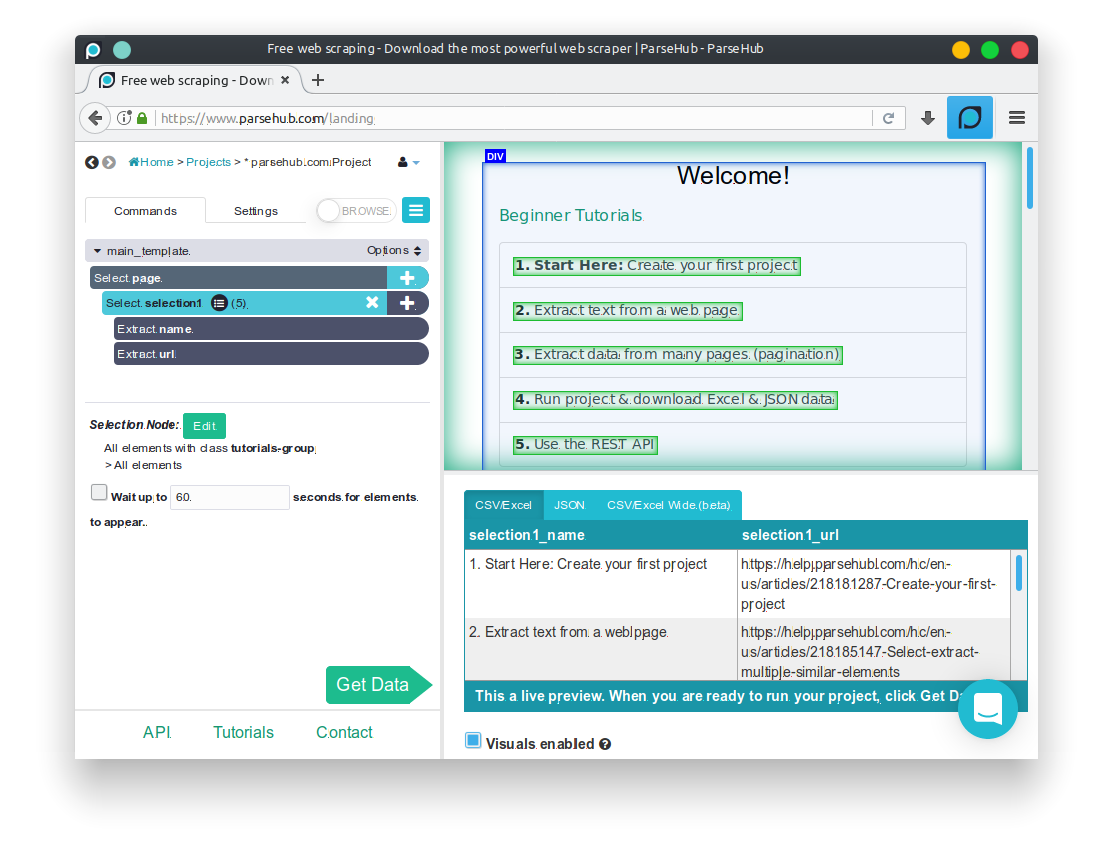
\includegraphics[width=\linewidth]{images/ParseHub.png}
	\caption{ParseHub\cite[snímek pořídil autor]{parsehub}}
	\label{fig:parseHub}
\end{figure}


\subsection{Octoparse}
\textbf{Výhody:}
\begin{itemize}
	\item výběr dat jak pomocí klikání (inteligentní hledání vzorců/podobností na základě prvních dvou kliknutí), tak pomocí XPath nebo regulárních výrazů
	\item nástroj obsahuje hotové šablony, které mohou velmi urychlit práci
	\item pestrá paleta možností (branch judgment, tvoření smyček apod.) -- dá se vytvořit téměř jakákoli logika procházení webu a extrakce dat
	\item lehký způsob, jak scrapování automatizovat
	\item možnost řídit tasky přes API (a získávat tak data taktéž přes API); data jdou nahrát rovnou i do lokální databáze
\end{itemize}
\textbf{Nevýhody:}
\begin{itemize}
	\item nutnost stažení aplikace (která je navíc pouze pro Windows)
	\item těžkopádné a pomalé ovládání, neintuitivní rozhraní
	\item tutoriál je v~podstatě nic neříkající
	\item připravených šablon je jenom pár a jsou velmi konkrétní
\end{itemize}
\begin{figure}[h]
	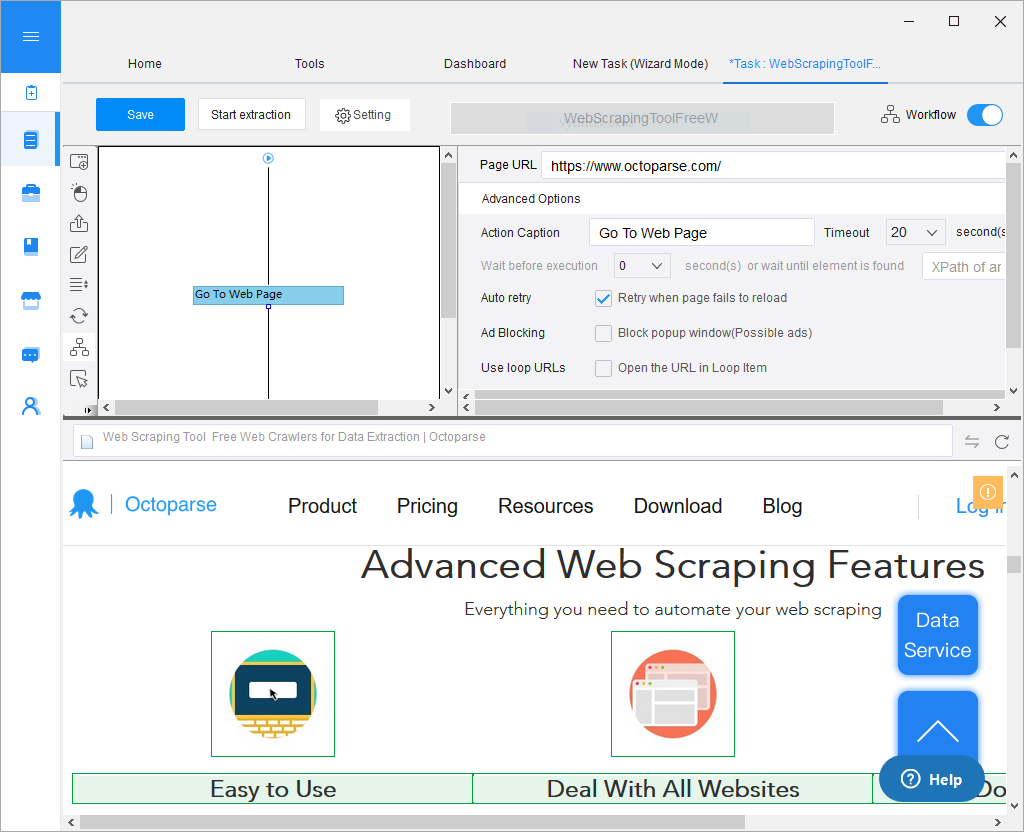
\includegraphics[width=\linewidth]{images/Octoparse.png}
	\caption{Octoparse\cite[snímek pořídil autor]{octoparse}}
	\label{fig:octoparse}
\end{figure}


\newpage
\subsection{WebScaper}
\begin{figure}
	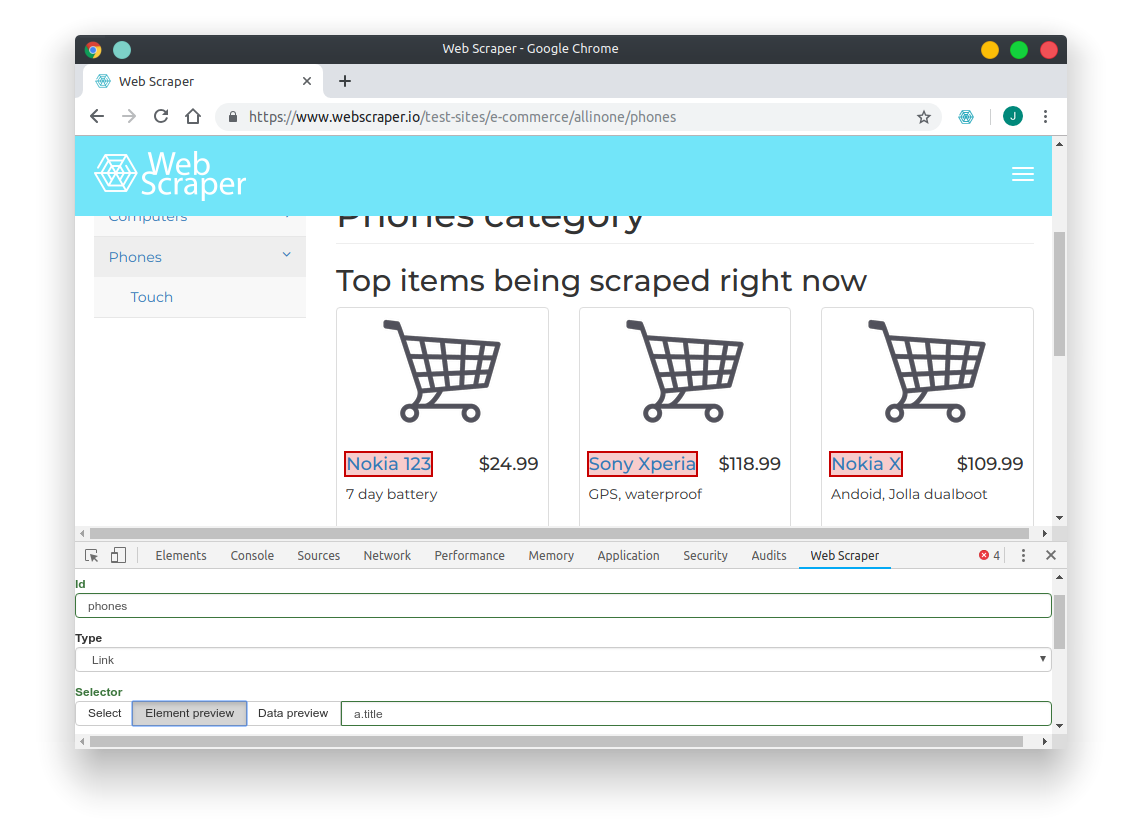
\includegraphics[width=\linewidth]{images/WebScraper.png}
	\caption{WebScraper\cite[snímek pořídil autor]{webscraper}}
	\label{fig:webScraper}
\end{figure}
\textbf{Výhody:}
\begin{itemize}
	\item jednoduchá instalace (jedná se pouze o~rozšíření do prohlížeče Google Chrome); scrapování probíhá skrze vývojářskou konzoli
	\item výběr dat pomocí klikání (inteligentní hledání vzorců/podobností na základě prvních dvou kliknutí)
	\item tutoriály jsou formou videí -- jednoduché, rychlé a naprosto postačující
	\item různé typy elementů, které vybíráme (text, odkaz, scroll down), takže lze celkem snadno projít celou doménu
	\item možnost získání dat různými formami -- přes API, jako CSV/XLS nebo do Dropboxu
	\item klávesové zkratky při výběru elementů velmi usnadňují práci
	\item možnost využít jejich cloud k~automatizaci celého procesu
	\item oproti konkurenci nabízí přehledné rozhraní, rychlé a jednoduché používání
\end{itemize}
\textbf{Nevýhody:}
\begin{itemize}
	\item nutnost používat Google Chrome, což pro některé uživatele může být překážka
	\item nelze vyhledávat podle klíčových slov ani podle HTML nebo CSS, tudíž všechno se musí manuálně naklikat
\end{itemize}


\subsection{Dexi.io}
\begin{figure}[h]
	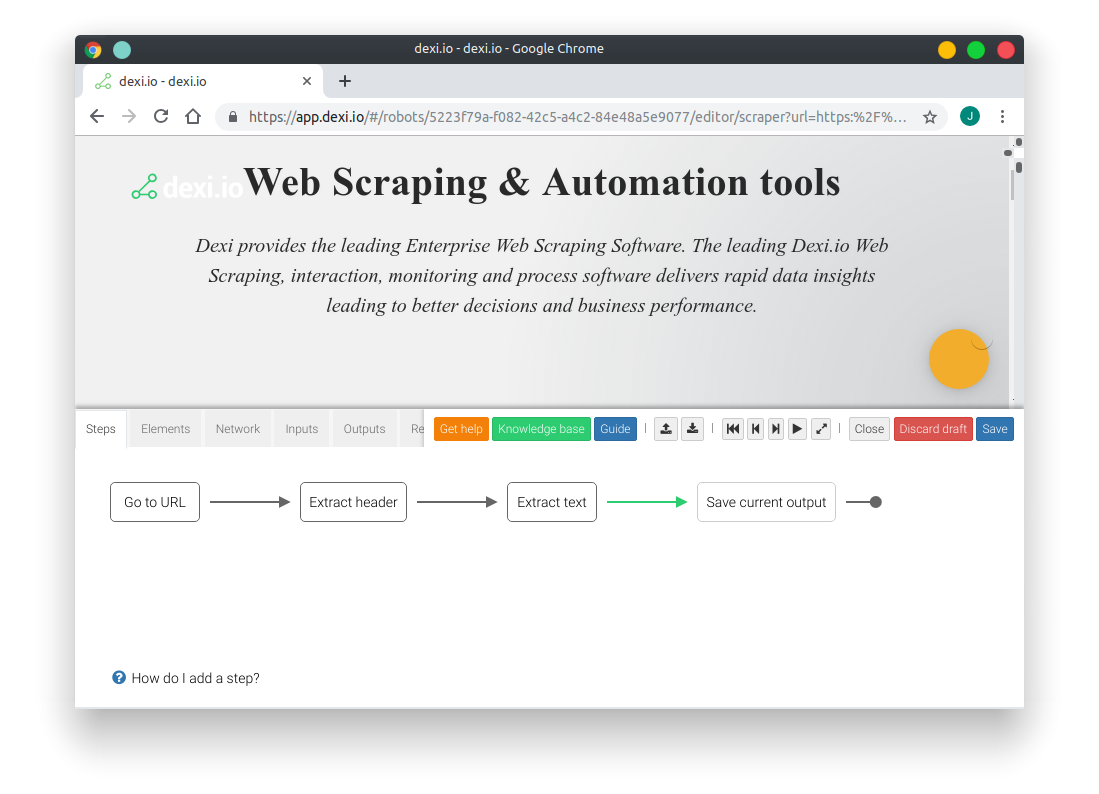
\includegraphics[width=\linewidth]{images/Dexiio.png}
	\caption{Dexi.io\cite[snímek pořídil autor]{dexio}}
	\label{fig:dexi.io}
\end{figure}
\textbf{Výhody:}
\begin{itemize}
	\item bez nutnosti stahování aplikace -- vše se ovládá přes webové rozhraní
	\item výběr dat jak pomocí klikání (inteligentní hledání vzorců/podobností na základě prvních dvou kliknutí), tak pomocí HTML, CSS nebo textové shody
	\item mnoho návodů dostupných na stránkách, interaktivní rádce přímo při scrapování
	\item všechny možné druhy kliknutí, takže lze lehce projít celou doménu
	\item možnost exportovat data do CSV, JSON, XLS, získat přes API, poslat do Google Drive, Google Sheets nebo Amazon S3
	\item různé módy aplikace -- scraping, crawler, pipes (skládání menších scrape botů) a autobot (extrahování z~více stránek najednou se stejným rozložením); možnost takto automatizovat celý proces.
	\item nápomocné jsou různé addony (např. na obcházení Captchy)
\end{itemize}
\textbf{Nevýhody:}
\begin{itemize}
	\item široká nabídka možností, a tak chvílí trvá, než se člověk zorientuje
	\item placený nástroj, zadarmo je dostupná pouze týdenní zkušební verze
	\item úvodní tutoriál je velmi strohý a žádné velké seznámení s~nástrojem se nekoná
\end{itemize}


\subsection{Data Scraper}
\textbf{Výhody:}
\begin{itemize}
	\item jednoduchá instalace (jedná se pouze o~rozšíření do prohlížeče Google Chrome).
	\item velmi jednoduché ovládání a přehledné rozhraní
	\item výběr dat probíhá pomocí klikání
	\item klikáním se utváří JQuery selektor, který si uživatel může podle svého upravit a doladit tak drobné detaily, jež by jinak nutně zahltily uživatelské rozhraní (tedy je možné vyhledávat i podle HTML tagů, id, CSS selektorů -- zkrátka vše, co umí klasické JQuery)
	\item různé druhy kliknutí
	\item možnost spustit na stránce libovolný JavaScriptový kód v~rámci scrapování
\end{itemize}
\textbf{Nevýhody:}
\begin{itemize}
	\item nutnost používat Google Chrome, což pro některé uživatele může být překážka
	\item oproti ostatním nástrojům se může zdát velmi chudý na různé funkce
\end{itemize}
\begin{figure}
	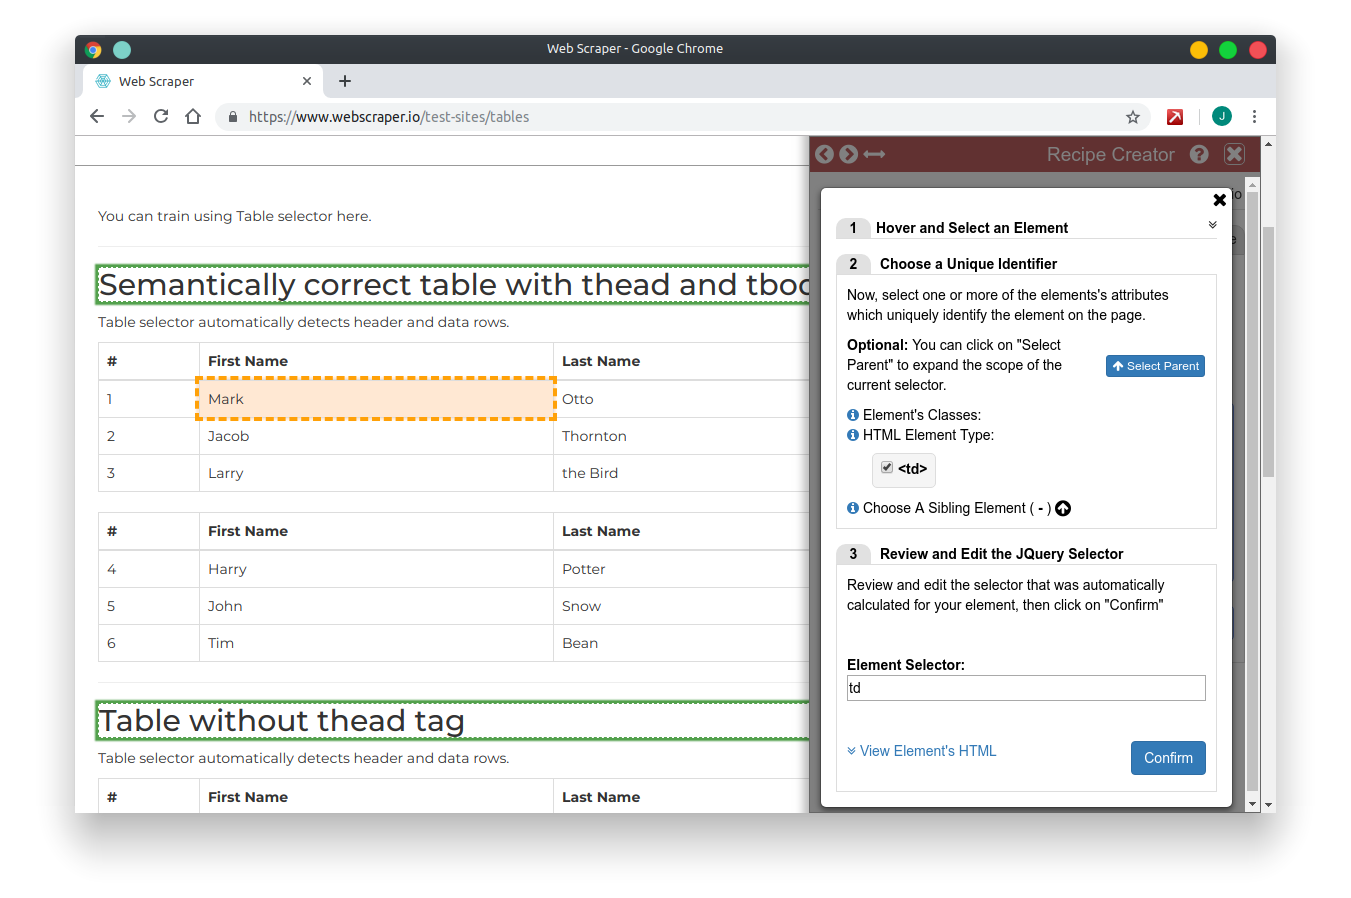
\includegraphics[width=\linewidth]{images/DataScraper.png}
	\caption{Data Scraper\cite[snímek pořídil autor]{data_scraper}}
	\label{fig:dataScraper}
\end{figure}

% ================================================================================================

\chapter{Návrh}

\section{Specifikace požadavků}
Jak jsme viděli v~předchozí analýze stávajících řešení, největšími neduhy, které se prolínají napříč valnou většinou aplikací, jsou \emph{těžkopádné uživatelské rozhraní}, \emph{neintuitivní ovládání} a \emph{rychlost} (nebo spíš pomalost), se kterou se uživatel dostane k~požadovaným datům. Pro aplikaci, jíž se tato práce zabývá, bude klíčové se výše zmíněným nedostatkům vyhnout a nabídnout jejich přesný opak. Také jsme se přesvědčili, že nejpříjemnější cestou je celou aplikaci ovládat přes webové rozhraní  \emph{bez nutnosti stahování a instalace}.

Na druhou stranu se lze u~konkurence i inspirovat. Za vyzdvižení stojí určitě \emph{různé druhy výběru dat} -- \emph{klikání} přímo na stránce spolu s~inteligentním hledáním podobných prvků jistě tvoří mocný mechanismus. Avšak je potřeba zajistit i ostatní způsoby výběru (jako je např. \emph{textová shoda, HTML tagy, CSS selektory}) pro případ, kdy je pouhé klikání zdlouhavé či nevyhovující. Rovněž široký výběr způsobů exportu dat, intuitivní klávesové zkratky a zooming in/out na prvky může uživatelům zpříjemnit práci s~nástrojem.

Neméně důležitou vlastností aplikace je také schopnost sebe sama kvalitně, ale svižně představit, \emph{seznámit uživatele s~používáním} a poskytnout mu alespoň pro začátek určité vodítko. Pro většinu ovládacích prvků by však mělo platit to stejné, co platí pro správný kód -- měly by být tzv. \emph{self-explanatory}. Tedy každému by mělo být na první pohled jasné, co který element dělá.

Pojďme si nyní všechny požadavky shrnout do několika bodů a rozdělit na funkční a nefunkční:

\subsection{Funkční požadavky}
\begin{itemize}
	\item uživatelské rozhraní se skládá z hlavní pracovní plochy, kde se bude nacházet uživatelem zadaná stránka a z postranního panelu, obsahující všechny ovládací prvky
	\item postranní panel skryje tlačítka, formuláře a ostatní elementy k ovládání aplikace do několika záložek -- tímto se na uživatele nevyvalí velké kvantum informací a možností najednou; podle potřeby si každý rozbalí tu možnost, kterou potřebuje
	\item hlavní činností uživatele bude výběr elementů na jím zadané webové stránce, ze kterých bude na konci procesu vyextrahován text; tento výběr bude probíhat následujícími způsoby:
	\begin{itemize}
		\item kliknutím myší na požadované elementy
		\item na základě textové shody; zde bude mít uživatel 4 možnosti na výběr:
		\begin{enumerate}
			\item Prvek bude vybrán, pokud jeho text začíná hledaným výrazem
			\item Prvek bude vybrán, pokud jeho text končí hledaným výrazem
			\item Prvek bude vybrán, pokud jeho text obsahuje hledaný výraz
			\item Prvek bude vybrán, pokud se jeho text přesně shoduje s hledaným výrazem
		\end{enumerate}
		\item pomocí CSS selektorů (tedy HTML tagy, třídy, id, hodnoty atributu, různé následnosti a vše ostatní, co CSS selektory umožňují, viz \href{https://www.w3schools.com/cssref/css_selectors.asp}{zde})
		\item na ovládacím panelu nalezneme i tlačítka s hotovými akcemi před-stavující šablonu pro nejpoužívanější operace (stažení všech obrázků ze stránky, všech emailových adres atd.)
	\end{itemize}
	\item pokud vybraným prvkem bude $\left<img\right>$ HTML tag, bude místo jeho textu extrahován atribut \textsf{src} (tedy zdroj obrázku)
	\item po kliknutí na určitý prvek s přidrženou klávesou \textsf{Ctrl/control} se program pokusí vybrat všechny podobné prvky na základě předchozí selekce (tzv. \emph{auto-selection})
	\item mezi ovládacími prvky nalezneme tlačítka \textsf{undo} a \textsf{redo}, která umožní vracet zpět provedený výběr (například v situaci, kdy nesouhlasíme s výběrem auto-selectu)
	\item všechny vybrané prvky budou barevně odlišeny, aby bylo jasné, co už je připraveno k extrakci a co ještě ne
	\item k dispozici bude přibližování (otec) a oddalování (první potomek) momentálního výběru pomocí ikony $+$ a $-$, případně přesunutí výběru na předchozího/následujícího sourozence v DOMu (uživatel klikne na daný element a pomocí této funkce může traverzovat napříč zanořenými prvky oběma směry)
	\item data z vybraných elementů si bude možné kdykoli prohlédnout v tzv. \textit{preview} módu -- půjde o obyčejnou tabulku, ze které bude možné vymazat nevyhovující řádky (vymazáním řádku se odebere výběr všech relevantních prvků na stránce)
	\item získaná data půjdou exportovat do formátů JSON, CSV, XLS
\end{itemize}

\subsection{Nefunkční požadavky}
\begin{itemize}
	\item půjde o webovou aplikaci běžící v internetovém prohlížeči, tedy nebude nutná žádná instalace
	\item celý proces bude realizován na straně klienta -- tedy bude se jednat pouze o frontend, žádný backend server nebude k dispozici
	\item aplikace cílí primárně na celkový zážitek uživatele -- grafické rozhraní bude přehledné a co nejjednodušší, ovládání přímočaré a intuitivní
	\item čas, za který se uživatel dostane k požadovaným datům (tedy čas, který stráví vybíráním dat; nepočítáme čas potřebný ke stažení), bude co nejmenší
	\item čas nutný k samotné extrakci (od okamžiku, kdy uživatel klikne na tlačítko \textsf{Download}) nepřesáhne 5 vteřin
\end{itemize}

\subsection{Nice to have požadavky}
V předchozích dvou sekcích jsme si shrnuli, jaké požadavky by naše aplikace v každém případě měla splňovat a bez nichž by neměla vůbec být uvedena k dispozici uživatelům. Pak tu máme ale také požadavky, které rozhodně zlepšují celkovou kvalitu a pocit z nástroje samotného, avšak nejsou již pro nás vitální a pokud by se jejich implementace nepovedla, aplikace bude stále plně funkční a připravená k použití. Patří sem:
\begin{itemize}
	\item uživatelské rozhraní aplikace nabídne intuitivní klávesové zkratky pro usnadnění práce -- \textsf{Ctrl +} a \textsf{Ctrl -} obstará přibližování/oddalování momentálního výběru, \textsf{Ctrl n} a \textsf{Ctrl p} vybere předchozího/následujícího sourozence vybraného prvku
	\item postranní panel s ovládacími prvky půjde minimalizovat (zmenšit k přilehlé hraně tak, aby zabíral co nejméně místa a nepřekážel v manipulaci s webovou stránkou) nebo přesunout na protější stranu (např. v případě, že by zakrýval nějaké prvky na stránce)
	\item export dat realizovatelný i do Google Sheets, Google Drive, Dropbox
	\item interaktivní tutoriál, který v rychlosti představí práci s nástrojem
	\item na základě výběru dat uživatelem se vytvoří určitý filtr (textový řetězec), který může být ručně upraven -- půjde tak o alternativu pro zkušenější uživatele, aniž by se zaneslo uživatelské rozhraní přehršlí možností a celé se tak znepřehlednilo
\end{itemize}

% ------------------------------------------------------------------------------------------------

\section{Architektura systému}

% ------------------------------------------------------------------------------------------------

\section{Návrh uživatelského rozhraní}

% ================================================================================================


\chapter{Realizace}

\section{Použité technologie}

% ------------------------------------------------------------------------------------------------

\section{Možná řešení}

% ------------------------------------------------------------------------------------------------

\section{Zvolené řešení}

% ================================================================================================


\begin{conclusion}
	%sem napište závěr Vaší práce
\end{conclusion}

\bibliographystyle{csn690}
\bibliography{mybibliographyfile}

\begin{thebibliography}{99}
	\bibitem{web_scraping_def}
	VARGIU, Eloisa; URRU, Mirko. Exploiting web scraping in a collaborative filtering- based approach to web advertising. \textit{Artificial Intelligence Research} [online]. 2013, roč. 2, č. 1 [cit. 13. 4. 2019]. DOI: 10.5430/air.v2n1p44. ISSN 1927-6974. Dostupné z: \url{http://www.sciedu.ca/journal/index.php/air/article/view/1390/1115}.
	
	\bibitem{web_crawler_def}
	KOBAYASHI, Mei; TAKEDA, Koichi.Information Retrieval on the Web. \textit{ACM Computing Surveys} [online]. 2000, roč. 32, č. 2 [cit. 13. 4. 2019]. DOI: 10.1145/358923.358934. ISSN 0360-0300. Dostupné z: \url{https://dl.acm.org/citation.cfm?doid=358923.358934}.
	
	\bibitem{web_wanderer}
	World Wide Web Wanderer. In: \textit{History-Computer} [online] [cit 13. 4. 2019]. Dostupné z: \url{https://history-computer.com/Internet/Conquering/Wanderer.html}.
	
	\bibitem{web_scraping_history}
	Web Scraping: How It All Started And Will Be. In: \textit{Octoparse's blog} [online]. © 2019 Octopus Data Inc. [cit. 13. 4. 2019]. Dostupné z: \url{https://www.octoparse.com/blog/web-scraping-introduction}.
	
	\bibitem{computer_vision}
	ROUSH, Wade. Diffbot Is Using Computer Vision to Reinvent the Semantic Web. In: \textit{Xconomy} [online]. © 2007--2019, Xconomy [cit. 13. 4. 2019]. Dostupné z: \url{https://xconomy.com/san-francisco/2012/07/25/diffbot-is-using-computer-vision-to-reinvent-the-semantic-web/}.
	
	\bibitem{data_size}
	WASSÉN, Olivia. Big Data facts – How much data is out there?. In: \textit{NodeGraph} [online]. © 2019 NodeGraph [cit. 13. 4. 2019]. Dostupné z: \url{https://www.nodegraph.se/big-data-facts/}.
	
	\bibitem{data_mining}
	CLIFTON, Christopher. Data mining. In: \textit{Encyclopædia Britannica} [online]. ©2019 Encyclopædia Britannica, Inc. [cit. 13. 4. 2019]. Dostupné z: \url{https://www.britannica.com/technology/data-mining}.
	
	\bibitem{rozhovor}
	VAŠÍČEK, Libor. [osobní sdělení]. Advokát specializující se na ICT právo a autorské právo. Sídlo advokátní kanceláře Legal Partners, s.~r.~o., Záhořanského 1944/4, Praha 2. 29. března 2019.
	
	\bibitem{browse_wrap}
	KUNKEL, R. G. Recent developments in shrinkwrap, clickwrap and browsewrap licenses in the United States. \textit{MurUEJL} [online]. 2002, roč. 9, č. 3 [cit. 1. 4. 2019]. Dostupné z: \url{http://www5.austlii.edu.au/au/journals/MurUEJL/2002/34.html}.
	
	\bibitem{take_it_or_leave_it}
	What Is a Take It or Leave It Contract?. In: \textit{UpCounsel} [online]. © 2019 UpCounsel, Inc [cit. 1. 4. 2019]. Dostupné z: \url{https://www.upcounsel.com/take-it-or-leave-it-contract}.
	
	\bibitem{click_wrap}
	OBAR, Jonathan A.; OELDORF-HIRSCH, Anne. The Clickwrap: A Political Economic Mechanism for Manufacturing Consent on Social Media. \textit{Social Media + Society} [online]. 2018, roč. 4, č. 3 [cit. 1. 4. 2019]. DOI: 10.1177/2056305118784770. ISSN 2056-3051. Dostupné z: \url{https://journals.sagepub.com/doi/10.1177/2056305118784770}.
	
	\bibitem{obcansky_zakon}
	ČESKO. Zákon č. 89/2012 Sb, občanský zákoník. In: \textit{Zákony pro lidi.cz} [online]. © AION CS 2010--2019 [cit. 30. 3. 2019]. Dostupné z: \url{https://www.zakonyprolidi.cz/cs/2012-89}.
	
	\bibitem{autorsky_zakon}
	ČESKO. Zákon č. 121/2000 Sb., o právu autorském, o právech souvisejících s právem autorským a o změně některých zákonů (autorský zákon). In: \textit{Zákony pro lidi.cz} [online]. © AION CS 2010--2019 [cit.~30.~3.~2019]. Dostupné z: \url{https://www.zakonyprolidi.cz/cs/2000-121}.
	
	\bibitem{polcak}
	POLČÁK, Radim. \textit{Právo informačních technologií}. Praha: Wolters Kluwer, 2018. Právní monografie (Wolters Kluwer ČR). 656 stran. ISBN 978-80-7598-045-8.
	
	\bibitem{ikaros}
	SMEJKAL, Ladislav. Právní ochrana databází v novém autorském zákoně. \textit{Ikaros} [online]. 2001, roč. 5, č. 3 [cit. 13. 4. 2019]. urn:nbn:cz:ik-10688. ISSN 1212-5075. Dostupné z: \url{http://ikaros.cz/node/10688}.
	
	\bibitem{C-444/02_1}
	Věc C-444/02, stanovisko generální advokátky ze dne 8. června 2004 ve věci Fixtures Marketing Ltd v. Organismos prognostikon agonon podosfairou AE (OPAP). In: \textit{EUR-Lex} [online]. © European Union, 1998--2019 [cit. 30. 3. 2019]. Dostupné z: \url{https://eur-lex.europa.eu/legal-content/CS/TXT/?uri=CELEX:62002CC0444}.
	
	\bibitem{C-444/02_2}
	Věc C-444/02, rozsudek Soudního dvora (velkého senátu) ze dne 9. listopadu 2004 ve věci Fixtures Marketing Ltd v. Organismos prognostikon agonon podosfairou AE (OPAP). In: \textit{EUR-Lex} [online]. © European Union, 1998--2019 [cit. 30. 3. 2019]. Dostupné z: \url{https://eur-lex.europa.eu/legal-content/CS/TXT/?uri=CELEX:62002CJ0444}.
	
	\bibitem{C-30/14}
	Věc C-30/14, rozsudek Soudního dvora (druhého senátu) ze dne 15. ledna 2015 ve věci Ryanair Ltd v. PR Aviation BV. In: \textit{EUR-Lex} [online]. © European Union, 1998--2019 [cit. 30. 3. 2019] .Dostupné z: \url{https://eur-lex.europa.eu/legal-content/CS/TXT/?uri=CELEX:62014CJ0030}.
	
	\bibitem{hiq_linkedin_1}
	Case 17-cv-03301-EMC, order granting plaintiff's motion for preliminary injunction, filed 08/14/17. In: \textit{The United States District Court for the Northern District of California} [online]. United States District Court [cit. 30. 3. 2019]. Dostupné z: \url{https://www.cand.uscourts.gov/filelibrary/3170/C-17-3301-hiQ-v.-LinkedIn-Order-Docket-No.-63.pdf}.
	
	\bibitem{linkedin_arg}
	WILLIAMS, Jamie. ‘Scraping’ Is Just Automated Access, and Everyone Does It. In: \textit{Electronic Frontier Foundation} [online]. Electronic Frontier Foundation [cit. 1. 4. 2019]. Dostupné z: \url{https://www.eff.org/deeplinks/2018/04/scraping-just-automated-access-and-everyone-does-it}
	
	\bibitem{public_forum}
	Forums, In: \textit{Legal Information Institute} [online]. Cornell Law School [cit. 30. 3. 2019]. Dostupné z: \url{https://www.law.cornell.edu/wex/forums}.
	
	\bibitem{hiq_linkedin_2}
	NARULA, Prayag. LinkedIn Vs. hiQ Ruling Casts A Long Shadow Over The Tech Industry. In: \textit{Forbes} [online]. © 2019 Forbes Media LLC [cit. 30. 3. 2019]. Dostupné z: \url{https://www.forbes.com/sites/forbestechcouncil/2017/09/20/linkedin-vs-hiq-ruling-casts-a-long-shadow-over-the-tech-industry}.
	
	\bibitem{facebook_venture_1}
	Case 13-17154, Facebook v. Vachani. In: \textit{United States Court of Appeals for the Ninth Circuit} [online]. [cit. 31. 3. 2019]. Dostupné z: \url{https://cdn.ca9.uscourts.gov/datastore/opinions/2016/07/12/13-17102.pdf}.
	
	\bibitem{facebook_venture_2}
	KERR, Orin. 9th Circuit: It’s a federal crime to visit a website after being told not to visit it. In: \textit{The Washington Post} [online]. © 1996--2019 The Washington Post [cit. 31. 3. 2019]. Dostupné z: \url{https://www.washingtonpost.com/news/volokh-conspiracy/wp/2016/07/12/9th-circuit-its-a-federal-crime-to-visit-a-website-after-being-told-not-to-visit-it/?noredirect=on\&utm_term=.ee6e01250364}.
	
	\bibitem{parsehub}
	PARSEHUB. \textit{ParseHub. Version 54.0.1} [software]. 2015 [cit. 13. 4. 2019]. Dostupné z: \url{https://www.parsehub.com/quickstart}.
	
	\bibitem{octoparse}
	OCTOPUS DATA INC. \textit{Octoparse. Version 7.1.2} [software]. 2018 [cit. 13. 4. 2019]. Dostupné z: \url{https://www.octoparse.com/download}.
	
	\bibitem{webscraper}
	WEBSCRAPER. \textit{WebScraper. Version 0.3.8.9} [software]. 2016 [cit. 13. 4. 2019]. Dostupné z: \url{https://chrome.google.com/webstore/detail/web-scraper/jnhgnonknehpejjnehehllkliplmbmhn}.
	
	\bibitem{dexio}
	DEXI APS. \textit{Dexi.io} [software] [cit. 13. 4. 2019]. Dostupné z: \url{https://app.dexi.io/}.
	
	\bibitem{data_scraper}
	 SOFTWARE INNOVATION LAB LLC. \textit{Data scraper. Version 3.299.84} [software]. 2015 [cit. 13. 4. 2019]. Dostupné z: \url{https://chrome.google.com/webstore/detail/data-scraper-easy-web-scr/nndknepjnldbdbepjfgmncbggmopgden}.
	
\end{thebibliography}

\appendix


% ================================================================================================


\chapter{Seznam použitých zkratek}
% \printglossaries
\begin{description}
	\item[HTML] HyperText Markup Language
	\item[DOM] 
	\item[XML] eXtensible Markup Language
	\item[API] Application Programming Interface
	\item[MIT] Massachusetts Institute of Technology
	\item[CSS] Cascading Style Sheets
	\item[CSV] Comma-Separated Values
	\item[IP] Internet Protocol
	\item[JSON] JavaScript Object Notation
	\item[XLS] formát souboru používaný aplikací Microsoft Excel
	\item[CFAA] Computer Fraud and Abuse Act
	\item[CAN-SPAM] Controlling the Assault of Non-Solicited Pornography and Marketing Act
\end{description}


% % % % % % % % % % % % % % % % % % % % % % % % % % % % 
% % Tuto kapitolu z výsledné práce ODSTRAŇTE.
% % % % % % % % % % % % % % % % % % % % % % % % % % % % 
% 
% \chapter{Návod k~použití této šablony}
% 
% Tento dokument slouží jako základ pro napsání závěrečné práce na Fakultě informačních technologií ČVUT v~Praze.
% 
% \section{Výběr základu}
% 
% Vyberte si šablonu podle druhu práce (bakalářská, diplomová), jazyka (čeština, angličtina) a kódování (ASCII, \mbox{UTF-8}, \mbox{ISO-8859-2} neboli latin2 a nebo \mbox{Windows-1250}). 
% 
% V~české variantě naleznete šablony v~souborech pojmenovaných ve formátu práce\_kódování.tex. Typ může být:
% \begin{description}
% 	\item[BP] bakalářská práce,
% 	\item[DP] diplomová (magisterská) práce.
% \end{description}
% Kódování, ve kterém chcete psát, může být:
% \begin{description}
% 	\item[UTF-8] kódování Unicode,
% 	\item[ISO-8859-2] latin2,
% 	\item[Windows-1250] znaková sada 1250 Windows.
% \end{description}
% V~případě nejistoty ohledně kódování doporučujeme následující postup:
% \begin{enumerate}
% 	\item Otevřete šablony pro kódování UTF-8 v~editoru prostého textu, který chcete pro psaní práce použít -- pokud můžete texty s~diakritikou normálně přečíst, použijte tuto šablonu.
% 	\item V~opačném případě postupujte dále podle toho, jaký operační systém používáte:
% 	\begin{itemize}
% 		\item v~případě Windows použijte šablonu pro kódování \mbox{Windows-1250},
% 		\item jinak zkuste použít šablonu pro kódování \mbox{ISO-8859-2}.
% 	\end{itemize}
% \end{enumerate}
% 
% 
% V~anglické variantě jsou šablony pojmenované podle typu práce, možnosti jsou:
% \begin{description}
% 	\item[bachelors] bakalářská práce,
% 	\item[masters] diplomová (magisterská) práce.
% \end{description}
% 
% \section{Použití šablony}
% 
% Šablona je určena pro zpracování systémem \LaTeXe{}. Text je možné psát v~textovém editoru jako prostý text, lze však také využít specializovaný editor pro \LaTeX{}, např. Kile.
% 
% Pro získání tisknutelného výstupu z~takto vytvořeného souboru použijte příkaz \verb|pdflatex|, kterému předáte cestu k~souboru jako parametr. Vhodný editor pro \LaTeX{} toto udělá za Vás. \verb|pdfcslatex| ani \verb|cslatex| \emph{nebudou} s~těmito šablonami fungovat.
% 
% Více informací o~použití systému \LaTeX{} najdete např. v~\cite{wikilatex}.
% 
% \subsection{Typografie}
% 
% Při psaní dodržujte typografické konvence zvoleného jazyka. České \uv{uvozovky} zapisujte použitím příkazu \verb|\uv|, kterému v~parametru předáte text, jenž má být v~uvozovkách. Anglické otevírací uvozovky se v~\LaTeX{}u zadávají jako dva zpětné apostrofy, uzavírací uvozovky jako dva apostrofy. Často chybně uváděný symbol "{} (palce) nemá s~uvozovkami nic společného.
% 
% Dále je třeba zabránit zalomení řádky mezi některými slovy, v~češtině např. za jednopísmennými předložkami a spojkami (vyjma \uv{a}). To docílíte vložením pružné nezalomitelné mezery -- znakem \texttt{\textasciitilde}. V~tomto případě to není třeba dělat ručně, lze použít program \verb|vlna|.
% 
% Více o~typografii viz \cite{kobltypo}.
% 
% \subsection{Obrázky}
% 
% Pro umožnění vkládání obrázků je vhodné použít balíček \verb|graphicx|, samotné vložení se provede příkazem \verb|\includegraphics|. Takto je možné vkládat obrázky ve formátu PDF, PNG a JPEG jestliže používáte pdf\LaTeX{} nebo ve formátu EPS jestliže používáte \LaTeX{}. Doporučujeme preferovat vektorové obrázky před rastrovými (vyjma fotografií).
% 
% \subsubsection{Získání vhodného formátu}
% 
% Pro získání vektorových formátů PDF nebo EPS z~jiných lze použít některý z~vektorových grafických editorů. Pro převod rastrového obrázku na vektorový lze použít rasterizaci, kterou mnohé editory zvládají (např. Inkscape). Pro konverze lze použít též nástroje pro dávkové zpracování běžně dodávané s~\LaTeX{}em, např. \verb|epstopdf|.
% 
% \subsubsection{Plovoucí prostředí}
% 
% Příkazem \verb|\includegraphics| lze obrázky vkládat přímo, doporučujeme však použít plovoucí prostředí, konkrétně \verb|figure|. Například obrázek \ref{fig:float} byl vložen tímto způsobem. Vůbec přitom nevadí, když je obrázek umístěn jinde, než bylo původně zamýšleno -- je tomu tak hlavně kvůli dodržení typografických konvencí. Namísto vynucování konkrétní pozice obrázku doporučujeme používat odkazování z~textu (dvojice příkazů \verb|\label| a \verb|\ref|).
% 
% \begin{figure}\centering
% 	
\includegraphics[width=0.5\textwidth, angle=30]{cvut-logo-bw}
% 	\caption[Příklad obrázku]{Ukázkový obrázek v~plovoucím prostředí}\label{fig:float}
% \end{figure}
% 
% \subsubsection{Verze obrázků}
% 
% % Gnuplot BW i barevně
% Může se hodit mít více verzí stejného obrázku, např. pro barevný či černobílý tisk a nebo pro prezentaci. S~pomocí některých nástrojů na generování grafiky je to snadné.
% 
% Máte-li například graf vytvořený v programu Gnuplot, můžete jeho černobílou variantu (viz obr. \ref{fig:gnuplot-bw}) vytvořit parametrem \verb|monochrome dashed| příkazu \verb|set term|. Barevnou variantu (viz obr. \ref{fig:gnuplot-col}) vhodnou na prezentace lze vytvořit parametrem \verb|colour solid|.
% 
% \begin{figure}\centering
% 	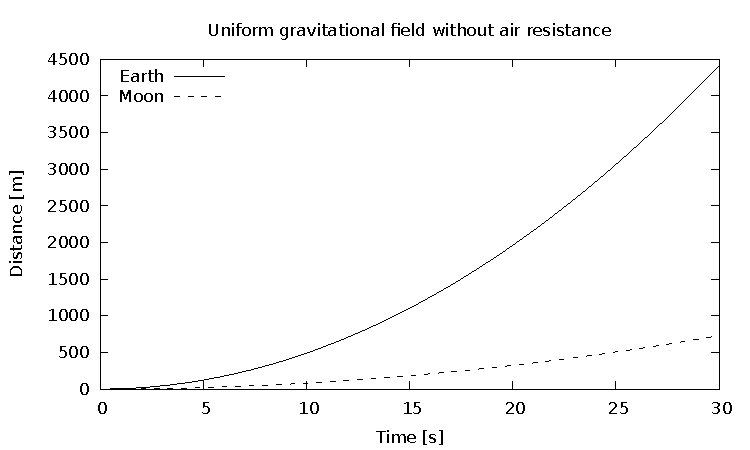
\includegraphics{gnuplot-bw}
% 	\caption{Černobílá varianta obrázku generovaného programem Gnuplot}\label{fig:gnuplot-bw}
% \end{figure}
% 
% \begin{figure}\centering
% 	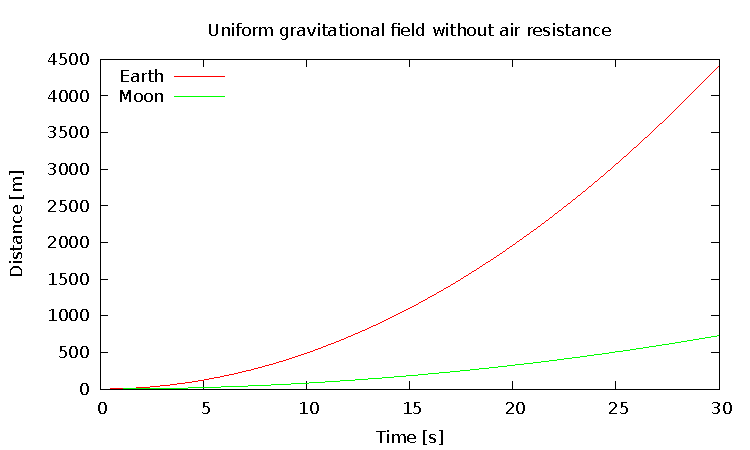
\includegraphics{gnuplot-col}
% 	\caption{Barevná varianta obrázku generovaného programem Gnuplot}\label{fig:gnuplot-col}
% \end{figure}
% 
% 
% \subsection{Tabulky}
% 
% Tabulky lze zadávat různě, např. v~prostředí \verb|tabular|, avšak pro jejich vkládání platí to samé, co pro obrázky -- použijte plovoucí prostředí, v~tomto případě \verb|table|. Například tabulka \ref{tab:matematika} byla vložena tímto způsobem.
% 
% \begin{table}\centering
% 	\caption[Příklad tabulky]{Zadávání matematiky}\label{tab:matematika}
% 	\begin{tabular}{|l|l|c|c|}\hline
% 		Typ		& Prostředí		& \LaTeX{}ovská zkratka	& \TeX{}ovská zkratka	\tabularnewline \hline \hline
% 		Text		& \verb|math|		& \verb|\(...\)|	& \verb|$...$|		\tabularnewline \hline
% 		Displayed	& \verb|displaymath|	& \verb|\[...\]|	& \verb|$$...$$|	\tabularnewline \hline
% 	\end{tabular}
% \end{table}
% 
% % % % % % % % % % % % % % % % % % % % % % % % % % % % 

\chapter{Obsah přiloženého CD}

%upravte podle skutecnosti

\begin{figure}
	\dirtree{%
		.1 readme.txt\DTcomment{stručný popis obsahu CD}.
		.1 exe\DTcomment{adresář se spustitelnou formou implementace}.
		.1 src.
		.2 impl\DTcomment{zdrojové kódy implementace}.
		.2 thesis\DTcomment{zdrojová forma práce ve formátu \LaTeX{}}.
		.1 text\DTcomment{text práce}.
		.2 thesis.pdf\DTcomment{text práce ve formátu PDF}.
		.2 thesis.ps\DTcomment{text práce ve formátu PS}.
	}
\end{figure}

\end{document}
